\documentclass[11pt,aspectratio=169, professionalfonts]{beamer}

\usepackage{tasks}
\usepackage{multicol}
\usepackage{amsmath}
\usepackage{amssymb}
\usepackage{vwcol}
\usepackage{python}
\usepackage[backend=biber, style=numeric,sorting=none]{biblatex}


\usepackage{tikz}
\usepackage{tikz-qtree}
%\usepackage{multirow}
\usepackage{wrapfig}
\usepackage{tcolorbox}
\usepackage{rotating}
%\usepackage{lmodern}% http://ctan.org/pkg/lm
\usepackage{anyfontsize}
\usepackage{algorithm,algorithmic}
%\usepackage[ruled,vlined]{algorithm2e}
%\usepackage{mathptmx}
%\usepackage{mathtools}
%\usepackage{pgfplots}
%\usepackage{pgfplotstable}
%\usepackage{outlines}
\usepackage{venndiagram}
% \DeclareGraphicsExtensions{.pdf,.png}
\usepackage{listings}
%\usepackage{hhline}
\usepackage{hyperref}
\usepackage{soul, xcolor}
\usepackage{graphicx}
\usepackage{color, colortbl}
\usepackage{tikz}
\usepackage[absolute,overlay]{textpos}
%\usepackage{algpseudocode}
\usepackage{relsize}
\usepackage{venndiagram}
%\usepackage[framemethod=TikZ]{mdframed}
%\usepackage{xparse}
%\usepackage{mdframed}
% \usepackage{accents}
% \usepackage[T1]{fontenc}
%\usepackage{transparent}
%\usepackage{varwidth}
% \usepackage{mwe} % provides example image

% \usepackage{emoji}
% \setemojifont{Apple Color Emoji}  % Optional
\definecolor{gold}{RGB}{255,215,0}
\definecolor{myblue}{rgb}{0.0,0.125,0.294}
\definecolor{beamer_title_color}{rgb}{1.0, 0.576,0.0}%\usepackage{enumitem}
\normalfont
%\input{/Users/ram/Documents/GitHub/NLProc/Latex/ColorCodes.tex}
% Override palette coloring with secondary
\setbeamercolor{subsection in head/foot}{,fg=white}

\setbeamercolor{normal text}{fg=white,bg=black}

\setbeamercolor{structure}{fg=white}
\setbeamercolor{definition}{fg=white}

%\setbeamercolor{alerted text}{fg=red!85!black}

%\setbeamercolor{item projected}{use=item,fg=black,bg=item.fg!35}

\setbeamercolor{note page}{bg=white}
\setbeamercolor{title}{bg=black, fg=yellow}
\setbeamercolor{author}{bg=black, fg=white}
\setbeamercolor{subtitle}{bg=black, fg=white}
\setbeamercolor{frametitle}{fg=orange,bg=black}
\setbeamertemplate{frametitle}{%
\usebeamerfont{frametitle} \MakeUppercase{\insertframetitle}%
\vphantom{g}% To avoid fluctuations per frame
\hrule% Uncomment to see desired effect, without a full-width hrule
\par% <-- added

{\color{white}\hrulefill}
}

\addtobeamertemplate{navigation symbols}{}{%
	\usebeamerfont{footline}%
	\usebeamercolor[fg=yellow]{footline}%
	\hspace{1em}%
	\insertframenumber/\inserttotalframenumber
}



\setbeamertemplate{footline}
{
	\leavevmode%
	\hbox{%
		\begin{beamercolorbox}[wd=.333333\paperwidth,ht=2.25ex,dp=1ex,center]{subsection in head/foot}%
			\usebeamerfont{subsection in head/foot}\insertsection
		\end{beamercolorbox}%
		\begin{beamercolorbox}[wd=.333333\paperwidth,ht=2.25ex,dp=1ex,center]{subsection in head/foot}%
			\usebeamerfont{title in head/foot}\insertshorttitle
		\end{beamercolorbox}%
		\begin{beamercolorbox}[wd=.333333\paperwidth,ht=2.25ex,dp=1ex,right]{section in head/foot}%
			\usebeamerfont{date in head/foot}\insertshortdate{}\hspace*{2em}
			\insertframenumber{} / \inserttotalframenumber\hspace*{2ex}
	\end{beamercolorbox}}%
	\vskip0pt%
}
\makeatother

\usetikzlibrary{chains,shapes}
\tikzstyle{MyText} = [text width=0.5cm,text centered]
\usetikzlibrary{decorations.text}
\setlength{\columnseprule}{0.2pt}
\def\columnseprulecolor{\color{yellow}}
\usepackage{nicefrac}
\usetikzlibrary{automata, shapes.geometric,circuits,positioning,shapes,arrows,fit,calc,decorations.pathmorphing,decorations}
% or whatever (possibly just delete it)

\usepackage[printwatermark=true]{xwatermark}



%\SetWatermarkText{\includegraphics{JCRLogo.png}}
%\setbeamertemplate{background}{
%	\tikz[overlay,remember picture]\node[opacity=0.04]at (current page.center){\includegraphics[width=4cm]{JCRLogo}};
%	}
\lstset{
backgroundcolor=\color{myblue},   % choose the background color; you must add \usepackage{color} or \usepackage{xcolor}; should come as last argument
basicstyle=\ttfamily\scriptsize,        % the size of the fonts that are used for the code
breakatwhitespace=false,         % sets if automatic breaks should only happen at whitespace
breaklines=false,                 % sets automatic line breaking
captionpos=b,                    % sets the caption-position to bottom
commentstyle=\color{green!25},    % comment style
deletekeywords={...},            % if you want to delete keywords from the given language
escapeinside={\%*}{*)},          % if you want to add LaTeX within your code
extendedchars=true,              % lets you use non-ASCII characters; for 8-bits encodings only, does not work with UTF-8
%frame=single,	                   % adds a frame around the code
keepspaces=true,                 % keeps spaces in text, useful for keeping indentation of code (possibly needs columns=flexible)
keywordstyle=\color{orange},       % keyword style
basicstyle=\small\ttfamily
morekeywords={*,...},            % if you want to add more keywords to the set
numbers=left,                    % where to put the line-numbers; possible values are (none, left, right)
numbersep=5pt,                   % how far the line-numbers are from the code
numberstyle=\tiny\color{cyan}, % the style that is used for the line-numbers
rulecolor=\color{white},         % if not set, the frame-color may be changed on line-breaks within not-black text (e.g. comments (green here))
showspaces=false,                % show spaces everywhere adding particular underscores; it overrides 'showstringspaces'
showstringspaces=false,          % underline spaces within strings only
showtabs=false,                  % show tabs within strings adding particular underscores
stepnumber=0,                    % the step between two line-numbers. If it's 1, each line will be numbered
stringstyle=\color{green},     % string literal style
tabsize=4,	                   % sets default tabsize to 2 spaces
%title=\lstname                   % show the filename of files included with \lstinputlisting; also try caption instead of title
belowskip=-5pt,
basicstyle=\ttfamily,
keywordstyle = \color{yellow},
language=Python,
}



\graphicspath{{Images/}}



\hypersetup{
colorlinks=true,
linkcolor=blue,
filecolor=magenta,
urlcolor=cyan,
}

\urlstyle{same}

\newsavebox\mybox

\newwatermark*[
angle=0,
allpages=true,
scale=0.1,
xpos=-5.75,
ypos=0
]{\usebox\mybox}


\tikzstyle{mybox} = [draw=white, fill=blue!75, very thick,
rectangle, rounded corners, inner sep=10pt, inner ysep=10pt]
\tikzstyle{fancytitle} =[draw=white,fill=blue!75, text=white, ellipse, very thick]



\newcommand{\ffbox}[1]{%
	{% open a group for a local setting
		\setlength{\fboxsep}{-2\fboxrule}% the rule will be inside the box boundary
		\fbox{\hspace{1.2pt}\strut#1\hspace{1.2pt}}% print the box, with some padding at the left and right
	}% close the group
}

\tikzset{
	NNnode/.pic={
		\pgfmathsetmacro\RecH{2}
		\pgfmathsetmacro\RecW{\RecH/10}
		\coordinate (-ll) at (-\RecW/2,-\RecH/2);
		\coordinate (-ur) at (\RecW/2,\RecH/2);
		\coordinate (-lr) at (-ll-|-ur);
		\coordinate (-ul) at (-ll|--ur);
		\path (-ul) -- (-ur) coordinate[midway] (-north);
		\path (-ll) -- (-lr) coordinate[midway] (-south);
		\path (-ll) -- (-ul) coordinate[midway] (-west);
		\path (-ur) -- (-lr) coordinate[midway] (-east);

		\begin{scope}[shift={(-\RecW/2,-\RecH/2)}]
			\draw (-ll) rectangle (-ur);
			\foreach \y in {0.05,0.5,0.75,0.85,0.95}
			\draw (0.5*\RecW,\RecH*\y) circle[radius=0.3*\RecW];
			\foreach \y in {0.275,0.625} {
				\fill (\RecW*0.4,\y*\RecH-0.1*\RecW) rectangle (0.6*\RecW,\y*\RecH-0.3*\RecW);
				\fill (\RecW*0.4,\y*\RecH+0.1*\RecW) rectangle (0.6*\RecW,\y*\RecH+0.3*\RecW);
			}
		\end{scope}
	}
}
\newenvironment{WrapText}[1][c]
{\wrapfigure{}{0.35\textwidth}\tcolorbox}
{\endtcolorbox\endwrapfigure}


\tikzstyle{decision} = [diamond, draw, text width=4.5em, text badly centered, node distance=3.5cm, inner sep=0pt]
\tikzstyle{block} = [rectangle, draw, text width=4em, text centered, rounded corners, minimum height=4em, node distance=0.5cm,minimum height=5em]
\tikzstyle{hidden} = [rectangle, draw, text width=0.5em, text centered, rounded corners, minimum height=2.5em, node distance=0.6cm,minimum height=2.5em,fill,red,opacity=0.85]
\tikzstyle{cloud} = [draw, ellipse, node distance=3.5cm, minimum height=2em]
\tikzstyle{line} = [draw, -latex']

\tikzstyle{vecArrow} = [thick, decoration={markings,mark=at position
	1 with {\arrow[semithick]{open triangle 60}}},
double distance=1.4pt, shorten >= 5.5pt,
preaction = {decorate},
postaction = {draw,line width=1.4pt, white,shorten >= 4.5pt}]
\tikzstyle{innerWhite} = [semithick, white,line width=1.4pt, shorten >= 4.5pt]

\DeclareMathOperator*{\argmin}{\arg\min}
\DeclareMathOperator*{\argmax}{\arg\max}

\tikzstyle{MyText} = [text width=0.5cm,text centered]


\newcommand\irregularline[2]{%
	let \n1 = {rand*(#1)} in
	+(0,\n1)
	\foreach \a in {0.1,0.2,...,#2}{
		let \n1 = {rand*(#1)} in
		-- +(\a,\n1)
	}
}

\usefonttheme{professionalfonts}
\setbeamercolor{frametitle}{fg=orange}
\setbeamerfont{frametitle}{size=\large}
\beamertemplatenavigationsymbolsempty


\newcommand*\circled[1]{\tikz[baseline=(char.base)]{
		\node[shape=circle,draw,inner sep=1pt] (char) {#1};}}

\setbeamertemplate{section in toc}{%
	\usebeamercolor[fg]{enumerate item}%
	\makebox[2em][l]{\circled{\inserttocsectionnumber}}%
	\parbox[t]{\dimexpr\linewidth-2em}{\inserttocsection}%
}
\setbeamercolor{item projected}{bg=orange}
\setbeamercolor*{item}{fg=orange}


\usepackage{xcolor}
\definecolor{c1}{rgb}{1,1,0} % blue
\definecolor{c2}{rgb}{1,1,1} % light blue
\definecolor{c3}{rgb}{1,1,0} % red blue
\hypersetup{
	linkcolor= {c1}, % internal links
	citecolor={c2}, % citations
	urlcolor={c3} % external links/urls
}

\setbeamercolor{background canvas}{bg=myblue}

%\setbeamercolor{note page}{bg=white}
\setbeamercolor{title}{bg=myblue, fg=gold}
\setbeamercolor{author}{bg=myblue, fg=white}
\setbeamercolor{subtitle}{bg=myblue, fg=white}
\setbeamercolor{frametitle}{fg=beamer_title_color,bg=myblue}
\addbibresource{/Users/ram/Documents/GitHub/NLProc/Latex/Bib/NLP.bib}

\logo{
	\begin{tikzpicture}[remember picture,overlay]
        \node[below left,inner sep=0pt] at (current page.north east) {
           \ifnum\thepage>1 
\includegraphics[width=1.00cm]{Images/TALogo}\fi
        };
      \end{tikzpicture}
      }

\newcommand{\clrtxt}[2]{\textcolor{#1}{#2}}
\newcommand{\keywordclr}[2][yellow]{\textcolor{#1}{#2}}
\newcommand{\headclr}[1]{\textcolor{cyan}{\textbf{\large #1}}\par}

\usepackage{fontspec}
\usepackage[defaultsans,scaled=.95]{opensans}
\renewcommand\seriesdefault{l}
\renewcommand\mddefault{l}
\renewcommand\bfdefault{sb}% or \renewcommand\bfdefault{m}

\usepackage{titlesec}

\title{Prompt Engineering\\RAG\\Reasoning}
\author{Your Name}
\date{\today}

\begin{document}

\maketitle

\begin{frame}[fragile]
\begin{block}{Questions}
\begin{itemize}
\item How does the prompt relate to the text it generates? Is there any logical reasoning involved in checking whether the context of the prompt corresponds to the generated text?
\item Is the reasoning engine module utilized in Gemini and other AI engines?
\item Given that the output is probabilistic and potentially multiple outcomes are possible, how does AI engine select the most probable output from the generated outputs?
\item Provide a comprehensive explanation of the vertex reasoning engine, accompanied by an illustrative example that elucidates its functionality.
\end{itemize}
\end{block}
\end{frame}
\begin{frame}
    \frametitle{Prompting in LLMs}
    \begin{itemize}
        \item \textbf{Prompting:} Using natural language instructions to guide LLMs.
        \item Enables tasks like:
            \begin{itemize}
                \item Translation
                \item Summarization
                \item Classification
            \end{itemize}
        \item  Crucial for effective interaction and desired outputs.
    \end{itemize}
    Image here
%    \includegraphics[width=0.5\textwidth]{example_prompt.png} % Replace with an actual image
\end{frame}

\begin{frame}
    \frametitle{In-Context Learning and Instruction Tuning}
    \begin{itemize}
        \item \textbf{In-Context Learning:} Prompts act as learning signals, improving performance without parameter updates.
        \item \textbf{Instruction Tuning:} Fine-tuning LLMs on instruction-response pairs to enhance instruction following.
        \item Both techniques improve LLM's ability to understand and respond to user requests.
    \end{itemize}
\end{frame}

\begin{frame}
    \frametitle{Model Safety Concerns}
    \begin{itemize}
        \item LLMs can generate harmful, false, or toxic content.
        \item Examples include:
            \begin{itemize}
                \item Unsafe advice
                \item Verbal attacks
                \item Hate speech
            \end{itemize}
        \item  Requires careful mitigation strategies.
    \end{itemize}
\end{frame}

\begin{frame}
    \frametitle{Model Alignment Techniques}
    \begin{itemize}
        \item \textbf{Safety Training:} Training models to avoid generating harmful content.
        \item \textbf{Preference Alignment:} Aligning model objectives with human goals.
        \item Common methods:
            \begin{itemize}
                \item Reinforcement Learning from Human Feedback (RLHF)
                \item Direct Preference Optimization (DPO)
            \end{itemize}
    \end{itemize}
\end{frame}

\begin{frame}
    \frametitle{Preference Alignment in Detail}
    \begin{itemize}
        \item A separate model is trained to assess the alignment of a candidate response with human preferences.
        \item This model guides the LLM towards generating more desirable outputs.
        \item  Crucial for ensuring that LLMs are helpful and harmless.
    \end{itemize}
    Image here
%    \includegraphics[width=0.5\textwidth]{preference_alignment.png} % Replace with an actual image
\end{frame}
\begin{frame}
\Huge\centering
Prompting
\end{frame}

\begin{frame}
    \frametitle{What is a Prompt?}
    \begin{itemize}
        \item A prompt is a text string issued to a language model.
        \item It guides the model to perform a specific task.
        \item The model generates tokens iteratively, conditioned on the prompt.
        \item Prompt engineering is the process of crafting effective prompts.
    \end{itemize}
\end{frame}

\begin{frame}{Overview}
  \begin{itemize}
    \item Tokenization
    \item Embedding
    \item Transformer Networks
    \item Contextual Understanding
    \item Language Generation
  \end{itemize}
\end{frame}

\begin{frame}{Tokenization}
  \begin{itemize}
    \item Breaking text into smaller units (tokens).
    \item Tokens can be words, subwords, or characters.
    \item Transforms raw text into numerical format.
  \end{itemize}
\end{frame}

\begin{frame}{Embedding}
  \begin{itemize}
    \item Converting tokens into numerical vectors (embeddings).
    \item Embeddings capture semantic meaning.
    \item Similar meanings have close embeddings.
  \end{itemize}
\end{frame}

\begin{frame}{Transformer Networks}
  \begin{itemize}
    \item Neural network architecture for sequential data.
    \item Key component: Attention mechanism.
    \item Attention weighs the importance of different tokens.
    \item Enables understanding of context.
  \end{itemize}
\end{frame}

\begin{frame}{Contextual Understanding}
  \begin{itemize}
    \item Transformer processes embedded tokens.
    \item Attention builds contextual understanding.
    \item Understanding represented by neuron activation patterns.
  \end{itemize}
\end{frame}

\begin{frame}{Language Generation}
  \begin{itemize}
    \item Predicting the next token in the sequence.
    \item Based on contextual understanding and learned patterns.
    \item Probability of each token is calculated.
    \item Process repeated iteratively.
  \end{itemize}
\end{frame}

\begin{frame}{Mathematical Formulation (Simplified)}
  \begin{itemize}
    \item Embeddings: $v_i \in \mathbb{R}^d$
    \item Attention:
      \begin{equation*}
        \text{Attention}(Q, K, V) = \text{softmax}\left(\frac{QK^T}{\sqrt{d_k}}\right)V
      \end{equation*}
    \item Probability distributions over vocabularies.
  \end{itemize}
\end{frame}
\begin{frame}{Solution Verification}
\begin{center}
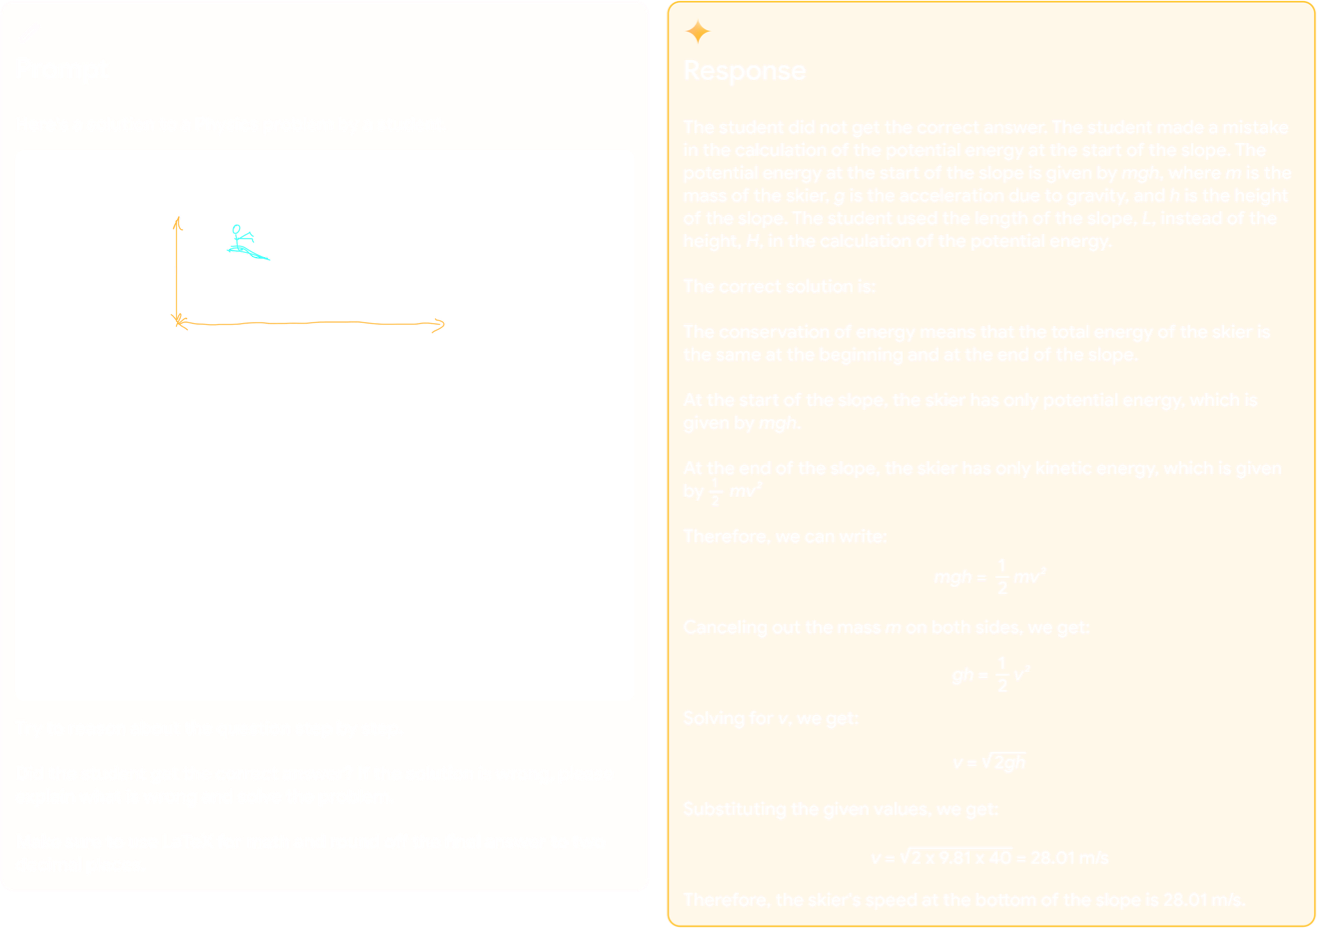
\includegraphics[width=0.7\linewidth]{Images/VerificationOfSolutionPrompt}
\\
Reference: \href{https://storage.googleapis.com/deepmind-media/gemini/gemini_1_report.pdf}{Gemini: A Family of Highly Capable
Multimodal Models}
\end{center}

\end{frame}
\begin{frame}[fragile]
    \frametitle{Prompting for Sentiment Classification}
    \begin{itemize}
        \item Task: Classify the sentiment of a hotel review.
        \item Example Review (BLT Corpus):
        \begin{verbatim}
Did not like the service that I was provided, when
I entered the hotel. I also did not like the
area, in which the hotel was located. Too much
noise and events going on for me to feel relax.

        \end{verbatim}
    \end{itemize}
\end{frame}

\begin{frame}[fragile]
    \frametitle{Crafting the Prompt}
    \begin{itemize}
        \item Append an incomplete statement to the review:
        \begin{verbatim}
Did not like the service that I was provided, when
 I entered the hotel. I also did not like the
 area, in which the hotel was located. Too much
 noise and events going on for me to feel relax.
 In short, our stay was:

        \end{verbatim}
        \item This prompt provides context for the LLM.
    \end{itemize}
\end{frame}

\begin{frame}
    \frametitle{LLM Completions}
    \begin{itemize}
        \item The LLM completes the statement by generating tokens.
        \item Examples of completions:
        \begin{itemize}
            \item "... not a pleasant one. The staff at the front desk were not welcoming or friendly, and seemed disinterested in providing good customer service."
            \item "... uncomfortable and not worth the price we paid. We will not be returning to this hotel."
        \end{itemize}
    \end{itemize}
\end{frame}

\begin{frame}
    \frametitle{Mapping Completions to Sentiment}
    \begin{itemize}
        \item Negative completions reflect the negative sentiment of the review.
        \item Map completions to predefined sentiment classes (e.g., negative, positive).
        \item Example mappings:
        \begin{itemize}
            \item \texttt{\{excellent $\rightarrow$ positive\}}
            \item \texttt{\{did not like $\rightarrow$ negative\}}
        \end{itemize}
    \end{itemize}
\end{frame}


\begin{frame}
    \frametitle{Prompting for General Tasks}
    \begin{itemize}
        \item LLMs can perform various tasks with appropriate contextual nudges.
        \item For tasks like summarization and translation, we need reusable prompts.
        \item \textbf{Templates:} Task-specific prompting text with input slots.
    \end{itemize}
\end{frame}

\begin{frame}
    \frametitle{Basic Prompt Templates}
    \begin{itemize}
        \item \textbf{Summarization:} \texttt{\{input\}; tldr;}
        \item \textbf{Translation:} \texttt{\{input\}; translate to French:}
        \item \textbf{Sentiment:} \texttt{\{input\}; Overall, it was}
        \item \textbf{Fine-Grained Sentiment:} \texttt{\{input\}; What aspects were important in this review?}
        \item \texttt{\{input\}} represents the input text.
    \end{itemize}
\end{frame}

\begin{frame}
    \frametitle{Instantiated Prompts}
    \begin{itemize}
        \item Templates are applied to inputs to create filled prompts.
        \item Example using the hotel review:
        \begin{itemize}
            \item \textbf{Summarization:} \texttt{Did not like the service...relax. tldr;}
            \item \textbf{Translation:} \texttt{Did not like the service...relax. translate to French:}
            \item \textbf{Sentiment:} \texttt{Did not like the service...relax. Overall, it was}
        \end{itemize}
        \item These are ready to be used with an LLM.  (See Figure 12.1 in your original document for example outputs)
    \end{itemize}
\end{frame}

\begin{frame}
    \frametitle{Prompt Design Principles}
    \begin{itemize}
        \item Input followed by text to be completed is a common pattern.
        \item This constrains the generation effectively.
        \item \textbf{Bad Example:} \texttt{Translate English to French: Did not like the service...}
        \item This prompt is ambiguous and may not produce a translation.
        \item Prompts should be designed unambiguously.
    \end{itemize}
\end{frame}

\begin{frame}[fragile]
    \frametitle{Constraining Prompts Further}
    \begin{itemize}
        \item Specify the set of possible answers in the prompt.
        \item Example for sentiment analysis:
        \begin{verbatim}
Human: Do you think that "input" has negative or positive sentiment?
Choices:
(P) Positive
(N) Negative
Assistant: I believe the best answer is:
        \end{verbatim}
        \item This provides even stronger guidance to the LLM.
    \end{itemize}
\end{frame}
\begin{frame}{Prompt Templates}
  \begin{itemize}
    \item Templates provide structure and context to prompts.
    \item They guide LLMs to generate specific types of responses.
    \item We'll explore templates using the hotel feedback example.
  \end{itemize}
\end{frame}

\begin{frame}{Template 1: Simple Complaint Template}
  \textbf{Template:} "I experienced [issue] at [location/time]. Specifically, [details]."
  \begin{itemize}
    \item \textbf{Example:} "I experienced poor service at check-in. Specifically, the process was slow and staff was unhelpful."
    \item \textbf{Example:} "I disliked the hotel's location. Specifically, it was too noisy."
  \end{itemize}
\end{frame}

\begin{frame}{Template 2: Detailed Feedback Template}
  \textbf{Template:} "I am writing to express my dissatisfaction with [aspect]. [Details]. As a result, [impact]."
  \begin{itemize}
    \item \textbf{Example:} "I am writing to express my dissatisfaction with the check-in service. The process was slow and the staff was unhelpful. As a result, I felt frustrated."
    \item \textbf{Example:} "I am writing to express my dissatisfaction with the hotel's location. There was constant noise from street events. As a result, I couldn't relax."
  \end{itemize}
\end{frame}

\begin{frame}{Template 3: Structured Problem-Solution Template}
    \textbf{Template:} "Problem: [issue]. Details: [details]. Recommendation: [solution]."
    \begin{itemize}
        \item \textbf{Example}: "Problem: Slow check-in. Details: 30-minute wait, unhelpful staff. Recommendation: Improve check-in efficiency and staff training."
        \item \textbf{Example}: "Problem: Noisy location. Details: Constant street events. Recommendation: Provide soundproof rooms or warn guests about the noise."
    \end{itemize}
\end{frame}

\begin{frame}{Template 4: Emotional Impact Template}
    \textbf{Template:} "I felt [emotion] due to [issue] at [location/time]. [Details]."
    \begin{itemize}
        \item \textbf{Example}: "I felt frustrated due to the slow check-in process. The staff was unhelpful and I waited for 30 minutes."
        \item \textbf{Example}: "I felt stressed due to the noisy location. Constant street events made it impossible to relax."
    \end{itemize}
\end{frame}

\begin{frame}{Applying Multiple Templates}
    \begin{itemize}
        \item Templates can be combined for comprehensive feedback.
        \item Example: "Problem: Slow check-in and noisy location. Details: 30-minute wait, unhelpful staff, constant street events. I felt frustrated and stressed. Recommendation: Improve efficiency, train staff, and address noise issues."
    \end{itemize}
\end{frame}

\begin{frame}{Benefits of Templates}
    \begin{itemize}
        \item \textbf{Consistency:} Ensures uniform structure across prompts.
        \item \textbf{Clarity:} Guides LLMs to generate specific responses.
        \item \textbf{Efficiency:} Reduces the time needed to craft effective prompts.
    \end{itemize}
\end{frame}


\begin{frame}{Connecting Prompts and Generated Text}
  \begin{itemize}
    \item How do LLMs ensure generated text aligns with the prompt?
    \item Is there logical reasoning involved?
  \end{itemize}
\end{frame}

\begin{frame}{Pattern Recognition and Statistical Relationships}
  \begin{itemize}
    \item LLMs trained on massive datasets.
    \item They recognize statistical relationships between words.
    \item Given a prompt, they find matching patterns.
    \item Prediction of "what comes next" based on likelihood.
  \end{itemize}
\end{frame}

\begin{frame}{Contextual Understanding Through Attention}
  \begin{itemize}
    \item Transformer architecture with attention mechanism.
    \item Attention weighs importance of prompt parts.
    \item Model focuses on relevant information.
    \item Maintains context throughout generation.
  \end{itemize}
\end{frame}

\begin{frame}{Probabilistic Generation}
  \begin{itemize}
    \item Generates text by predicting next word's probability.
    \item Prediction based on prompt context and preceding words.
    \item Determines most likely word to follow.
  \end{itemize}
\end{frame}

\begin{frame}{Limitations of "Logical Reasoning"}
  \begin{itemize}
    \item LLMs don't possess true reasoning abilities.
    \item Rely on learned patterns, leading to inconsistencies.
    \item Can produce factually incorrect statements.
    \item Active research to improve logical reasoning.
  \end{itemize}
\end{frame}

\begin{frame}{How Context is Maintained}
  \begin{itemize}
    \item "Context window" limits preceding text consideration.
    \item Maintains running context for consistency.
    \item Context window limitations can affect coherence.
  \end{itemize}
\end{frame}

\begin{frame}{Probabilistic Output and Selection}
  \begin{itemize}
    \item LLMs generate probabilistic outputs.
    \item Multiple probable outcomes exist.
    \item How does the AI engine select the final output?
  \end{itemize}
\end{frame}

\begin{frame}{Probability Distributions}
  \begin{itemize}
    \item LLMs produce probability distributions over possible tokens.
    \item Each token has an associated probability score.
    \item Higher scores indicate more likely tokens.
  \end{itemize}
\end{frame}

\begin{frame}{Selection Strategies}
  \begin{itemize}
    \item \textbf{Greedy Decoding:}
      \begin{itemize}
        \item Selects the token with the highest probability at each step.
        \item Simple but can lead to suboptimal results.
      \end{itemize}
    \item \textbf{Sampling:}
      \begin{itemize}
        \item Randomly samples tokens based on their probabilities.
        \item Introduces diversity but can be inconsistent.
      \end{itemize}
    \item \textbf{Beam Search:}
      \begin{itemize}
        \item Keeps track of multiple promising sequences (beams).
        \item Selects the sequence with the highest overall probability.
        \item Balances quality and diversity.
      \end{itemize}
    \item \textbf{Top-k and Top-p Sampling:}
      \begin{itemize}
        \item Restricts sampling to the top k most probable tokens or tokens whose cumulative probability exceeds p.
        \item Controls diversity and reduces the risk of low-probability outputs.
      \end{itemize}
  \end{itemize}
\end{frame}

\begin{frame}{Post-Processing and Refinement}
  \begin{itemize}
    \item Selected output may undergo post-processing.
    \item Techniques like:
      \begin{itemize}
        \item Filtering for safety and relevance.
        \item Re-ranking based on additional criteria.
        \item Paraphrasing or editing for clarity.
      \end{itemize}
  \end{itemize}
\end{frame}

\begin{frame}{Factors Affecting Selection}
  \begin{itemize}
    \item Task requirements (e.g., creativity vs. accuracy).
    \item Model parameters (e.g., temperature).
    \item User preferences (e.g., length, style).
  \end{itemize}
\end{frame}


\begin{frame}{Prompt, RAG, and LLMs: A Symbiotic Relationship}
  \begin{itemize}
    \item Understanding the interaction between Prompts, Retrieval Augmented Generation (RAG), and Large Language Models (LLMs).
    \item Exploring the role of Gemini API, Vertex AI API, and seminal papers.
  \end{itemize}
\end{frame}

%%%%%%%%
\begin{frame}
\Huge
\centering
Retrieval Augmented Generation (RAG)
\end{frame}



\begin{frame}{Overview}
  \begin{itemize}
    \item Understanding the interaction between Prompts, Retrieval Augmented Generation (RAG), and Large Language Models (LLMs).
    \item Exploring the role of Gemini API, Vertex AI API, and seminal papers.
  \end{itemize}
\end{frame}

\begin{frame}{Prompts: The Starting Point}
  \begin{itemize}
    \item Prompts are the user's input, guiding the LLM's response.
    \item They define the task, context, and desired output.
    \item Effective prompts are crucial for accurate and relevant LLM outputs.
  \end{itemize}
\end{frame}

\begin{frame}{How do I get updated content with LLMs}
  \begin{itemize}
    \item LLMs like Gemini/ChapGPT/DeepSeek/LLama are trained on vast datasets, enabling them to generate human-like text.
    \item They excel at understanding and generating language, but can suffer from:
      \begin{itemize}
        \item Lack of up-to-date information.
        \item "Hallucinations" (generating factually incorrect information).
      \end{itemize}
  \end{itemize}
\end{frame}
\begin{frame}{RAG Overview}
\begin{center}
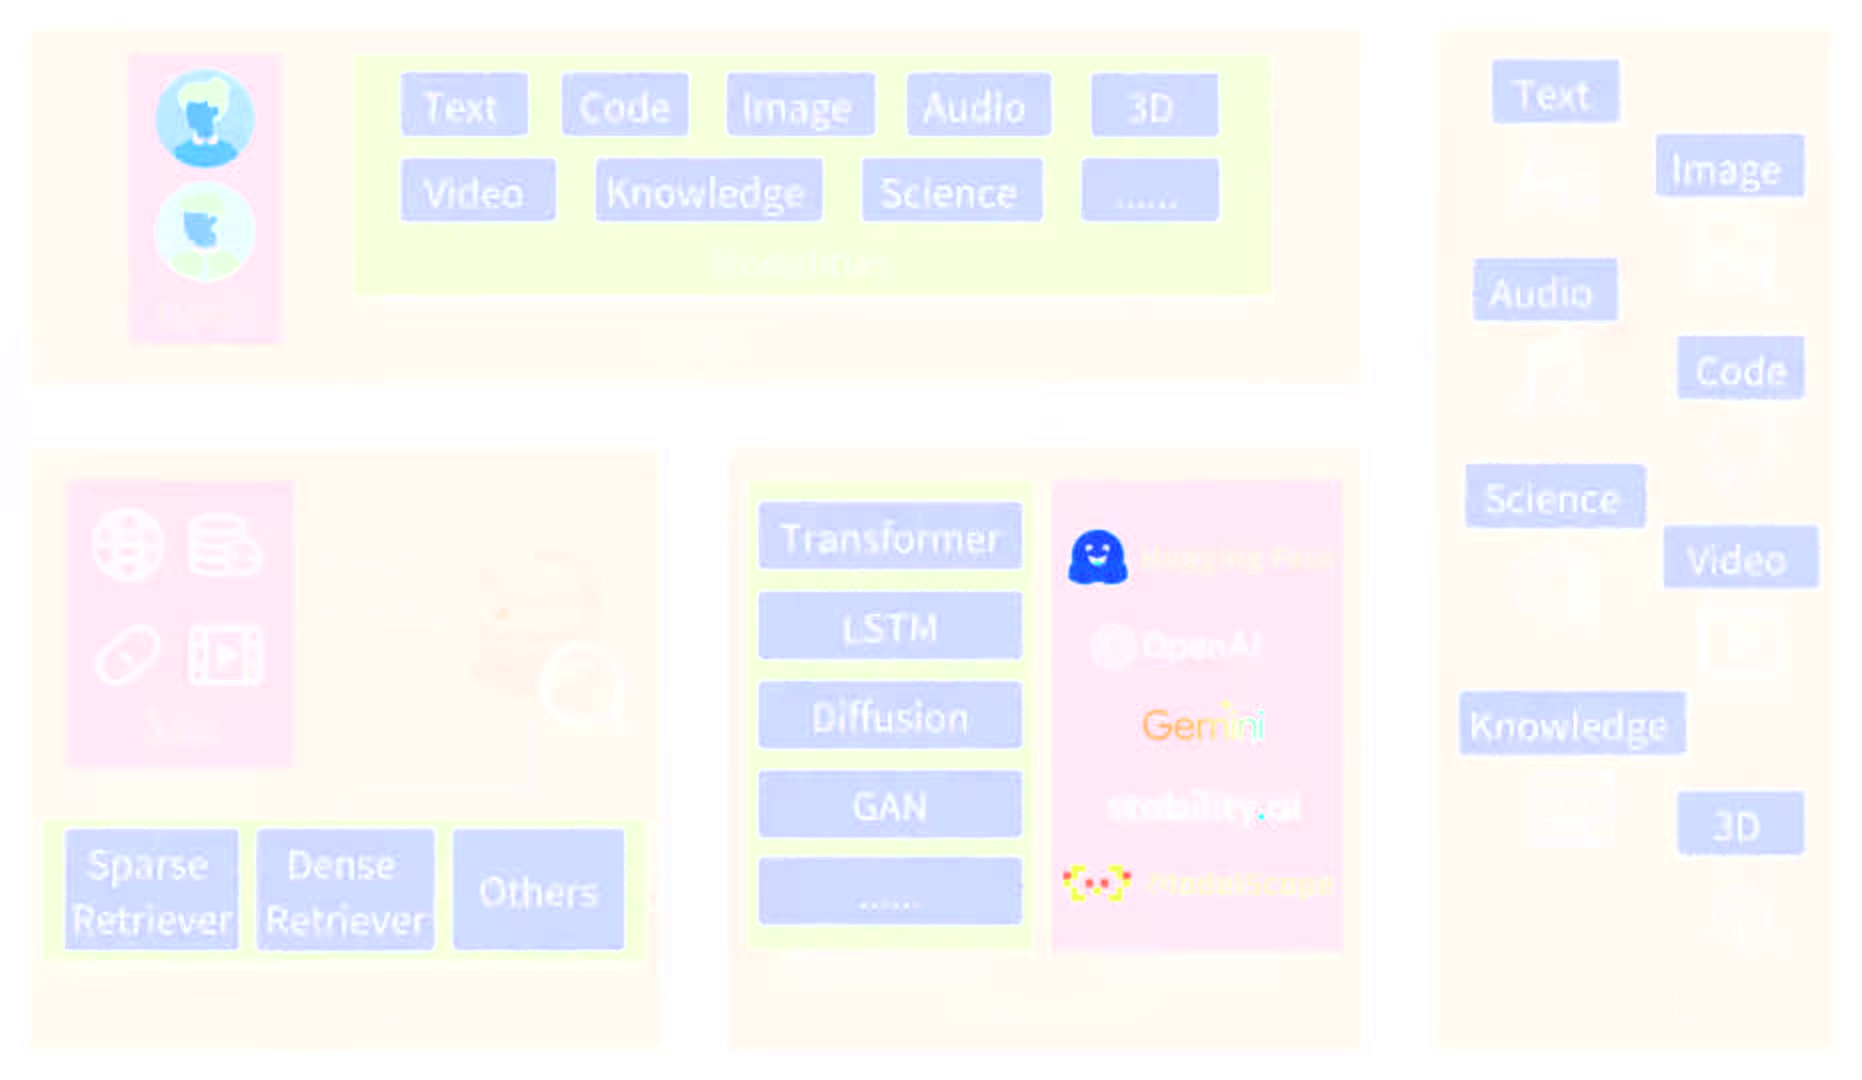
\includegraphics[width=0.9\linewidth]{Images/RAGOverview}
\end{center}

\end{frame}
\begin{frame}{Retrieval Augmented Generation (RAG)}
  \begin{itemize}
    \item RAG enhances LLMs by retrieving relevant information from external knowledge sources.
    \item It addresses the limitations of LLMs by providing access to up-to-date and domain-specific information.
    \item Key steps:
      \begin{itemize}
        \item Retrieval: Using an information retrieval engine to find relevant documents.
        \item Augmentation: Injecting the retrieved information into the prompt.
        \item Generation: LLM generates a response based on the augmented prompt.
      \end{itemize}
  \end{itemize}
\end{frame}

\begin{frame}{The Connection: Prompt + RAG + LLM}
  \begin{itemize}
    \item User provides a \textbf{prompt}.
    \item \textbf{RAG} system retrieves relevant information based on the prompt.
    \item Retrieved information is incorporated into an \textbf{augmented prompt}.
    \item \textbf{LLM} uses the augmented prompt to generate a response.
    \item This process ensures the response is grounded in external knowledge and contextually relevant.
  \end{itemize}
\end{frame}
\begin{frame}{}
\Huge
\centering
Reasoning with LLMS
\end{frame}
\begin{frame}{Reasoning Engines}
  \begin{itemize}
    \item Reasoning engines are systems designed to derive conclusions from given information.
    \item They use logical rules and inference mechanisms to process data.
    \item Traditionally, they have been rule-based systems.
    \item In the context of AI, they enhance decision-making and problem-solving.
  \end{itemize}
\end{frame}

\begin{frame}{Traditional Reasoning Engines}
  \begin{itemize}
    \item Rule-based systems: "If-then" logic.
    \item Well-defined rules for specific domains.
    \item Limitations:
      \begin{itemize}
        \item Difficulty handling ambiguity.
        \item Limited to predefined rules.
      \end{itemize}
  \end{itemize}
\end{frame}

\begin{frame}{Reasoning Engines in LLMs}
  \begin{itemize}
    \item Modern LLMs are integrating advanced reasoning capabilities.
    \item Moving beyond simple rule-based systems.
    \item Enhancing LLMs with:
      \begin{itemize}
        \item Contextual reasoning.
        \item Tool use.
        \item Agentic workflows.
      \end{itemize}
  \end{itemize}
\end{frame}

\begin{frame}{Contextual Reasoning}
  \begin{itemize}
    \item LLMs analyze context using vast training data.
    \item Attention mechanisms process and weigh information.
    \item Enables understanding of complex relationships.
    \item Example: Answering questions based on the surrounding text.
  \end{itemize}
\end{frame}
\begin{frame}{Introduction}
  \begin{itemize}
    \item Reasoning engines involve logical inference.
    \item Mathematical frameworks can formalize these processes.
    \item This treatment focuses on propositional logic and first-order logic.
  \end{itemize}
\end{frame}

\begin{frame}{Propositional Logic}
  \begin{itemize}
    \item Propositions: Statements that are either true or false.
    \item Connectives: $\neg$ (negation), $\wedge$ (conjunction), $\vee$ (disjunction), $\rightarrow$ (implication), $\leftrightarrow$ (biconditional).
    \item Truth tables: Define the semantics of connectives.
    \item Inference rules: Modus ponens, modus tollens, etc.
  \end{itemize}
\end{frame}

\begin{frame}{Mathematical Representation}
  \begin{itemize}
    \item Let $P, Q$ be propositions.
    \item Modus ponens: If $P$ and $P \rightarrow Q$ are true, then $Q$ is true.
    \item Symbolically: $(P \wedge (P \rightarrow Q)) \rightarrow Q$.
    \item This can be verified using truth tables.
  \end{itemize}
\end{frame}

\begin{frame}{First-Order Logic}
  \begin{itemize}
    \item Extends propositional logic with predicates, quantifiers, and variables.
    \item Predicates: Represent properties or relations.
    \item Quantifiers: $\forall$ (for all), $\exists$ (there exists).
    \item Variables: Represent objects in a domain.
  \end{itemize}
\end{frame}

\begin{frame}{Mathematical Representation (First-Order)}
  \begin{itemize}
    \item Example: "All humans are mortal."
    \item Let $H(x)$ be "x is a human" and $M(x)$ be "x is mortal."
    \item Symbolically: $\forall x (H(x) \rightarrow M(x))$.
    \item Inference: If $H(John)$ is true, then $M(John)$ is true.
  \end{itemize}
\end{frame}

\begin{frame}{Reasoning as Inference}
    \begin{itemize}
        \item Inference involves deriving new knowledge from existing knowledge.
        \item Mathematical logic provides formal rules for inference.
        \item Automated theorem proving: Algorithms that perform logical inference.
    \end{itemize}
\end{frame}

\begin{frame}{Connecting with LLMs}
    \begin{itemize}
        \item LLMs can generate and manipulate logical expressions.
        \item Integrating formal logic with LLMs enhances reasoning capabilities.
        \item Techniques:
        \begin{itemize}
            \item Symbolic reasoning with LLM generated logical rules.
            \item LLMs used to generate or verify logical proofs.
            \item Knowledge graphs and logical queries.
        \end{itemize}
    \end{itemize}
\end{frame}

\begin{frame}{Mathematical Reasoning in LLMs}
    \begin{itemize}
        \item LLMs can be trained on datasets containing logical expressions and proofs.
        \item Techniques like neural theorem proving are being explored.
        \item LLMs can use external tools to perform logical inference.
        \item Example: LLM generating logical queries for a knowledge graph.
    \end{itemize}
\end{frame}


\begin{frame}{Seminal Paper References}
  \begin{itemize}
    \item \textbf{Lewis et al. (2020):} "Retrieval-Augmented Generation for Knowledge-Intensive NLP Tasks." \cite{lewis2020retrieval}
    \item \textbf{Komeili et al. (2021):} "Internet-Augmented Language Models through Interactive Retrieval." \cite{komeili2021internet}
    \item P. Zhao, et al,  ``Retrieval-
    augmented generation for ai-generated content: A survey'', \href{https://arxiv.org/abs/2402.19473}{3} 2024.
  \end{itemize}
\end{frame}

\begin{frame}{Google Cloud Ecosystem}
    \begin{itemize}
        \item \textbf{Vertex AI API:}
        \begin{itemize}
            \item Provides tools and services for building and deploying AI models, including RAG implementations.
            \item Offers access to LLMs like Gemini and information retrieval capabilities.
        \end{itemize}
        \item \textbf{Gemini API:}
        \begin{itemize}
            \item Allows developers to integrate Gemini's capabilities into their applications.
            \item Can be used in conjunction with Vertex AI Search for RAG implementations.
        \end{itemize}
    \end{itemize}
\end{frame}

\begin{frame}{RAG in Practice}
    \begin{itemize}
        \item User asks a question.
        \item Vertex AI Search retrieves relevant documents.
        \item Gemini API uses the retrieved documents to generate an informed answer.
        \item Vertex AI reasoning engine can orchestrate this process.
    \end{itemize}
\end{frame}

%\begin{frame}{Conclusion}
%  \begin{itemize}
%    \item Prompts, RAG, and LLMs work synergistically to create powerful AI applications.
%    \item RAG addresses the limitations of LLMs by providing access to external knowledge.
%    \item Google Cloud's Vertex AI and Gemini APIs provide the tools for building RAG-enabled applications.
%  \end{itemize}
%\end{frame}

%\begin{frame}{References}
%    \begin{thebibliography}{9}
%        \bibitem{lewis2020retrieval}
%        Lewis, P., Perez, E., Piktus, A., Petroni, F., Karpukhin, V., Goyal, N., ... & Riedel, S. (2020). Retrieval-augmented generation for knowledge-intensive NLP tasks. \textit{Advances in Neural Information Processing Systems}, \textbf{33}, 9459-9474.
%        \bibitem{komeili2021internet}
%        Komeili, M., Lewis, P., Shuster, K., Yih, W. T., & Riedel, S. (2021). Internet-augmented language models through interactive retrieval. \textit{arXiv preprint arXiv:2103.07567}.
%    \end{thebibliography}
%\end{frame}


%%%%%%%%%
\begin{frame}{Prompts: The Starting Point}
  \begin{itemize}
    \item Prompts are the user's input, guiding the LLM's response.
    \item They define the task, context, and desired output.
    \item Effective prompts are crucial for accurate and relevant LLM outputs.
  \end{itemize}
\end{frame}

\begin{frame}{Large Language Models (LLMs)}
  \begin{itemize}
    \item LLMs like Gemini are trained on vast datasets, enabling them to generate human-like text.
    \item They excel at understanding and generating language, but can suffer from:
      \begin{itemize}
        \item Lack of up-to-date information.
        \item "Hallucinations" (generating factually incorrect information).
      \end{itemize}
  \end{itemize}
\end{frame}

\begin{frame}{Retrieval Augmented Generation (RAG)}
  \begin{itemize}
    \item RAG enhances LLMs by retrieving relevant information from external knowledge sources.
    \item It addresses the limitations of LLMs by providing access to up-to-date and domain-specific information.
    \item Key steps:
      \begin{itemize}
        \item Retrieval: Using an information retrieval engine to find relevant documents.
        \item Augmentation: Injecting the retrieved information into the prompt.
        \item Generation: LLM generates a response based on the augmented prompt.
      \end{itemize}
  \end{itemize}
\end{frame}

\begin{frame}{The Connection: Prompt + RAG + LLM}
  \begin{itemize}
    \item User provides a \textbf{prompt}.
    \item \textbf{RAG} system retrieves relevant information based on the prompt.
    \item Retrieved information is incorporated into an \textbf{augmented prompt}.
    \item \textbf{LLM} uses the augmented prompt to generate a response.
    \item This process ensures the response is grounded in external knowledge and contextually relevant.
  \end{itemize}
\end{frame}

\begin{frame}{Seminal Paper References}
  \begin{itemize}
    \item \textbf{Lewis et al. (2020):} "Retrieval-Augmented Generation for Knowledge-Intensive NLP Tasks." \cite{lewis2020retrieval}
    \item \textbf{Komeili et al. (2021):} "Internet-Augmented Language Models through Interactive Retrieval." \cite{komeili2021internet}
  \end{itemize}
\end{frame}

\begin{frame}{Google Cloud Ecosystem}
    \begin{itemize}
        \item \textbf{Vertex AI API:}
        \begin{itemize}
            \item Provides tools and services for building and deploying AI models, including RAG implementations.
            \item Offers access to LLMs like Gemini and information retrieval capabilities.
        \end{itemize}
        \item \textbf{Gemini API:}
        \begin{itemize}
            \item Allows developers to integrate Gemini's capabilities into their applications.
            \item Can be used in conjunction with Vertex AI Search for RAG implementations.
        \end{itemize}
    \end{itemize}
\end{frame}
%
\begin{frame}{RAG in Practice}
    \begin{itemize}
        \item User asks a question.
        \item Vertex AI Search retrieves relevant documents.
        \item Gemini API uses the retrieved documents to generate an informed answer.
        \item Vertex AI reasoning engine can orchestrate this process.
    \end{itemize}
\end{frame}

\begin{frame}{Conclusion}
  \begin{itemize}
    \item Prompts, RAG, and LLMs work synergistically to create powerful AI applications.
    \item RAG addresses the limitations of LLMs by providing access to external knowledge.
    \item Google Cloud's Vertex AI and Gemini APIs provide the tools for building RAG-enabled applications.
  \end{itemize}
\end{frame}

\begin{frame}{References}
    \begin{thebibliography}{9}
        \bibitem{lewis2020retrieval}
        Lewis, P., Perez, E., Piktus, A., Petroni, F., Karpukhin, V., Goyal, N., ... \& Riedel, S. (2020). Retrieval-augmented generation for knowledge-intensive NLP tasks. \textit{Advances in Neural Information Processing Systems}, \textbf{33}, 9459-9474.
        \bibitem{lewis2020retrieval}
        Lewis, P., Perez, E., Piktus, A., Petroni, F., Karpukhin, V., Goyal, N., ... \& Riedel, S. (2020). Retrieval-augmented generation for knowledge-intensive NLP tasks. \textit{Advances in Neural Information Processing Systems}, \textbf{33}, 9459-9474.
        \bibitem{komeili2021internet}
                Komeili, M., Lewis, P., Shuster, K., Yih, W. T., \& Riedel, S. (2021). Internet-augmented language models through interactive retrieval. \textit{arXiv preprint arXiv:2103.07567}.
                \bibitem{guu2020realm}
                Guu, K., Lee, K., Tung, Z.,\& Chang, M. W. (2020). REALM: Retrieval-augmented language model pre-training. \textit{arXiv preprint arXiv:2002.08909}.

    \end{thebibliography}
\end{frame}



\end{document}